\section{Videoplayer}
\label{sec:videoplayer}

\subsection{Ziel}
In einem ersten Schritt, vor der Realisierung des Fahrsimulator, wird ein Videoplayer ralisiert. Das Ziel dabei ist der Aufbau und Test der Anbindung der Eingabehardware an unser Programm. Bei der Betätigung des Gaspedals im Cockpit soll das aufgenommene Video schneller abgespielt werden. Bei der Betätigung des Bremspedals dementsprechend langsamer. Der Videoplayer soll so aufgebaut werden, dass Komponenten davon auch im Fahrsimulator wiederverwendet werden können. Die ETH Zürich besitzt bereits Videos, die sich gut dafür eigenen. Um Experimente mit diesen Videos durchführen zu können, müssen Eingaben, die der Proband im Cockpit mach, mit der aktuellen Position des Videos abgespeichert werden. Dies dient zur späteren Auswertung der Experimente.
\\
\subsection{Systembeschreibung}

Um einzelne Komponenten des Videoplayer wiederverwenden zu können, wird das System möglichst gleich wie das des Fahrsimulators aufgebaut. Dieser Aufbau wird anhand der Abbildung \ref{Systembeschreibung Videoplayer} illustriert. Blau markiert sind neu entwickelte Komponenten des Videoplayers. Die Eingaben im Cockpit werden von einem LabVIEW-Programm über eine USB-Schnittstelle eingelesen. Die eingelesenen Parameter werden, zusammen mit einem Timestamp, von LabVIEW in ein UDP-Paket verpackt und über einen UDP-Socket gesendet. Das Paket wird von einem UDP-Listener empfangen und gelesen. Dieser speichert die Daten ab und hält sie für das Hauptprogramm bereit. Das Hauptprogramm liest die gespeicherten Parameter aus und interpretiert diese. Der \gls{mplayer}, der für das Abspielen der Videos verwendet wird, lässt sich durch Konsoleneingaben über die Standard-In-Pipe steuern. So wird ihm vom Videoplayer mitgeteilt, wie schnell das aktuelle Video abgespielt werden soll. Über die Standard-Out-Pipe gibt MPlayer die aktuelle Abspielposition zurück. Das Hauptprogramm wertet diese aus, ergänzt sie mit den Benutzereingaben und leitet sie über den UDP-Listener an LabVIEW weiter. Dort werden die Daten über einen zweiten UDP-Socket empfangen und für eine spätere Auswertung in ein Log-File gespeichert.
\newpage

% Bild für Systembeschreibung des Video Players
\begin{figure}[H]
\centering 
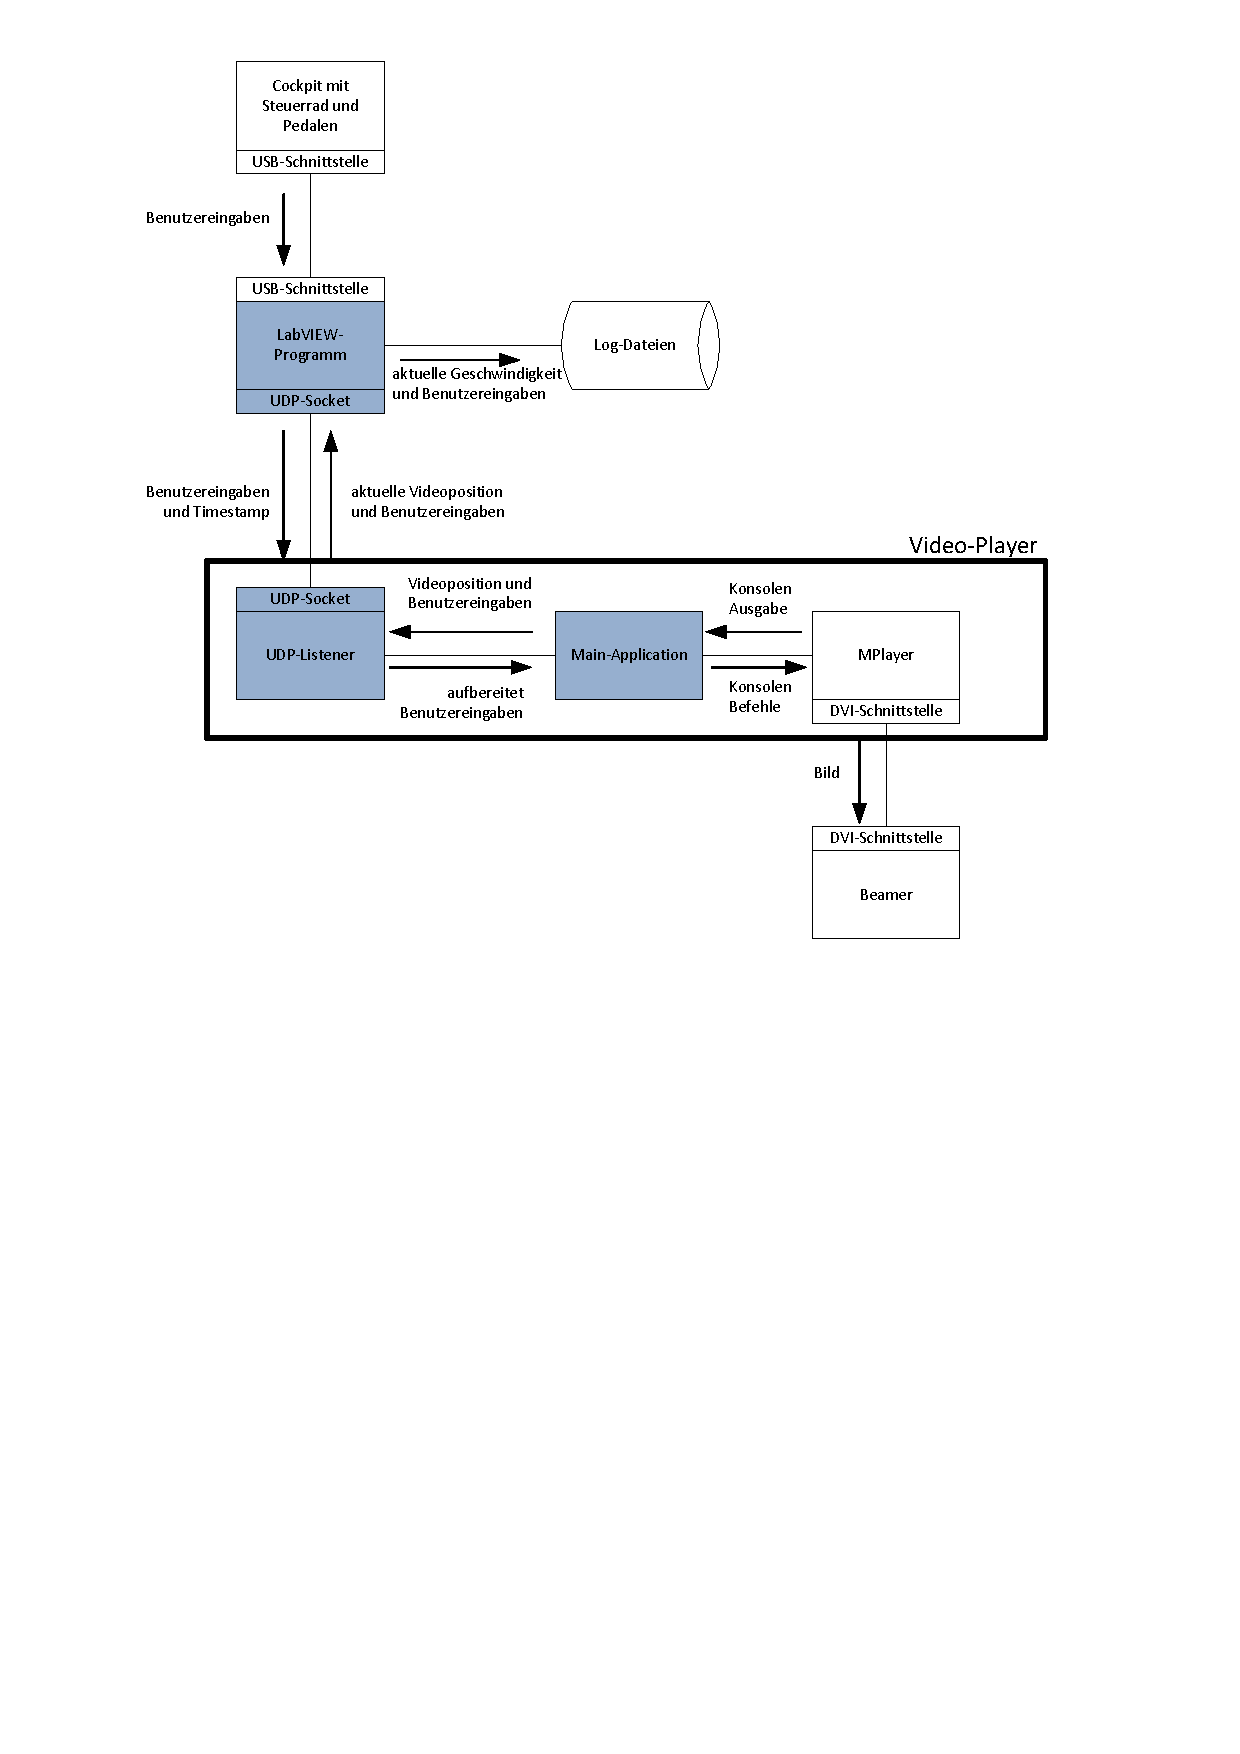
\includegraphics[width=0.8\linewidth]{src/Systembeschreibung_VideoPlayer.pdf}
\caption{Systembeschreibung Videoplayer} % Titel der Grafik
\label{Systembeschreibung Videoplayer} % Labelname
\end{figure}

\subsection{Realisierung}
Bei der Realisierung des Videoplayers wird der Fokus vorallem auf die Entwicklung der LabVIEW-Schnittstelle zu unserem Programm gelegt. Darum wird dieser Schritt nachfolgend ausführlich erklährt. Diese Schnittstelle wird auch für den Fahrsimulator selbst verwendet.

\subsubsection{LabVIEW-Schnittstelle}
\label{labview_schnittstelle}
Die Realisierung der LabVIEW Schnittstelle wird in zwei Teile unterteilt. Der erste Teil dient dazu, die Benutzereingaben einzulesen und an den UDP-Listener zu senden. Der zweite Teil befasst sich mit dem Empfangen von Daten, die vom UDP-Listener gesendet werden und deren Speicherung in ein Log-File.

\newpage 

% LabVIEW Screenshot, Daten senden
\begin{figure}[H]
\centering 
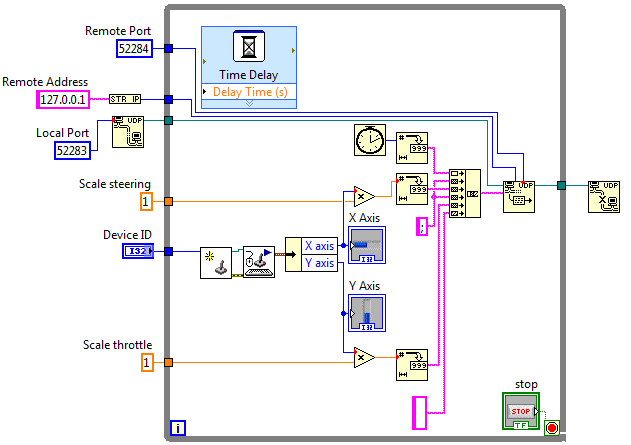
\includegraphics[width=1\linewidth]{src/labview_screenshot_videoplayer_daten_senden.png}
\caption{Einlesen und Versenden der Daten mit LabVIEW} % Titel der Grafik
\label{labview_screenshot_videoplayer_daten_senden} % Labelname
\end{figure}
Die Abbildung \ref{labview_screenshot_videoplayer_daten_senden} illustriert den Aufbau des LabVIEW-Programms, mit dem Eingaben vom Cockpit eingelesen und über einen UDP-Socket versendet werden. Das Verhalten des Programms kann über diverse Parameter geändert werden.\\
Die \textit{Remote Address} gibt an, an wen die UDP-Pakete gesendet werden. Da sich der UDP-Listener zur Zeit auf dem selben Rechner wie dieses Programm befindet, wählen wir hierfür die Localhost-Adresse 127.0.0.1. Für den \textit{Remote Port} wählen wir einen freien Port, hier 52284. Zusammen mit dem \textit{Local Port}, der uns eine Verbindungs-ID generiert, ist unsere Konfiguration für den UDP-Socket vollständig. Um die Komponenten im Cockpit ansprechen zu können, muss lediglich die richtige \textit{Device ID} gewählt werden. Die anderen Komponenten, die sich in der grauen Box befinden, werden in einer Schleife 100 mal pro Sekunde ausgeführt. Dieser Wert wird mit dem Element \textit{Time Delay} konfiguriert.\\
Aus dem Cockpit werden die Werte der x- und y-Achse des Joysticks eingelesen. Auf der y-Achse werden die Werte der beiden Pedalen abgebildet. Ein negativer Wert quantiviziert hierbei das Drücken des Gaspedals, ein positiver Wert das Drücken des Bremspedals. Die Intensität beider Pedalen wird im Positiven durch 32767 und im Negativen durch 32768 ganzzahlige Werte abgestuft. Ein voll gedrücktes Gaspedal entspricht also dem Wert -32768 auf der y-Achse und ein voll gedrücktes Bremspedal entspricht dem Wert 32767. Die x-Achse quantifiziert analog dazu den Einschlagswinkel des Steuerrades. Hierbei ist, wenn das Steuerrad sich in der neutralen Position befindet, der x-Wert null. Komplett nach rechts eingeschlagen beträgt der x-Wert 32767 und -32768 bei einem Einschlag nach links. Der x-Wert wird ebenfalls ausgelesen, ist aber im Video-Player nicht relevant. Die beiden Werte werden je mit einem separaten Faktor multipliziert, um eventuell eine Anpassung derjenigen vorzunehmen. Danach werden sie zusammen mit dem aktuellen Timestamp durch Semikolons voneinander getrennt, in das UDP-Paket gepackt und dann versendet. Bei Beendigung des Programms wird die Schleife verlassen und der UDP-Socket wieder geschlossen.

Die Abbildung \ref{labview_screenshot_videoplayer_daten_empfangen} illustriert den Aufbau des LabVIEW-Programms, mit dem die Daten vom Videoplayer empfangen und in ein Log-File gespeichert werden.\\
Es wird ein UDP-Socket geöffnet um ankommende Pakete zu empfangen. Der \textit{Local port} mit dem UDP-Verbindungskästchen generiert wieder eine Connection-ID, die für das Öffnen des UPD-Ports benötigt wird. Durch die Angaben von \textit{Maximum datagram size} und \textit{Timeout} wird der UPD-Socket so konfiguriert, dass er nur Pakete kleiner als 4096 Bytes empfängt und höchstens 500 ms auf das Eintreffen eines Pakets wartet. Ist die Übertragung des Pakets fehlerhaft oder dauert sie zu lange, wird abgebrochen und auf das nächste Paket gewartet. Der hierbei von LabVIEW erzeugte Fehler wird ignoriert.\\
Bei einer erfolgreichen Übertragung liegen die Daten als eine Zeichenkette vor. Die einzelnen Werte in der Zeichenkette sind mit Semikolons voneinander getrennt. Diese Zeichenkette wird jetzt weiterverarbeitet. Die beiden Filmstreifenfenster bewirken, dass die Aktionen im zweiten Fenster erst ausgeführt werden, wenn die im ersten Fenster erzeugten Daten vollständig vorliegen. Dies ist vorallem für den Timestamp, der wieder von der Uhr kommt, wichtig, da dieser erst erstellt werden darf, wenn das Packet gelesen wurde. Die Werte werden voneinander getrennt und die Semikolons gelöscht. Sie repräsentieren nun verschiedenste Eigenschaften des Systems. So ist zum Beispiel der dritte Wert die aktuelle Geschwindigkeit des Fahrzeuges. Dieser Wert wird benötigt um auf der Benutzeroberfläche die Geschwindgkeit in einem Tacho anzuzeigen. Zudem wird auch der vierte Wert benötigt um die aktuelle Abspielposition des Videos auszugeben. Alle Werte, inklusive der aktuellen Position von Pedalen und Steuerrad, werden nun, wieder getrennt durch Semikolons, zu einer Zeichenkette zusammengefügt. Diese wird dann laufend in einem File gespeichert. Die erste Zeile des Files ist ein Header und beschreibt die Felder. Er wird in der Abbildung \ref{labview_screenshot_videoplayer_daten_empfangen} unten links zusammengestellt. Nachdem die Schleife beendet wurde, werden UDP-Socket und File geschlossen.

\newpage

% LabVIEW Screenshot, Daten empfangen
\begin{figure}[H]
\centering 
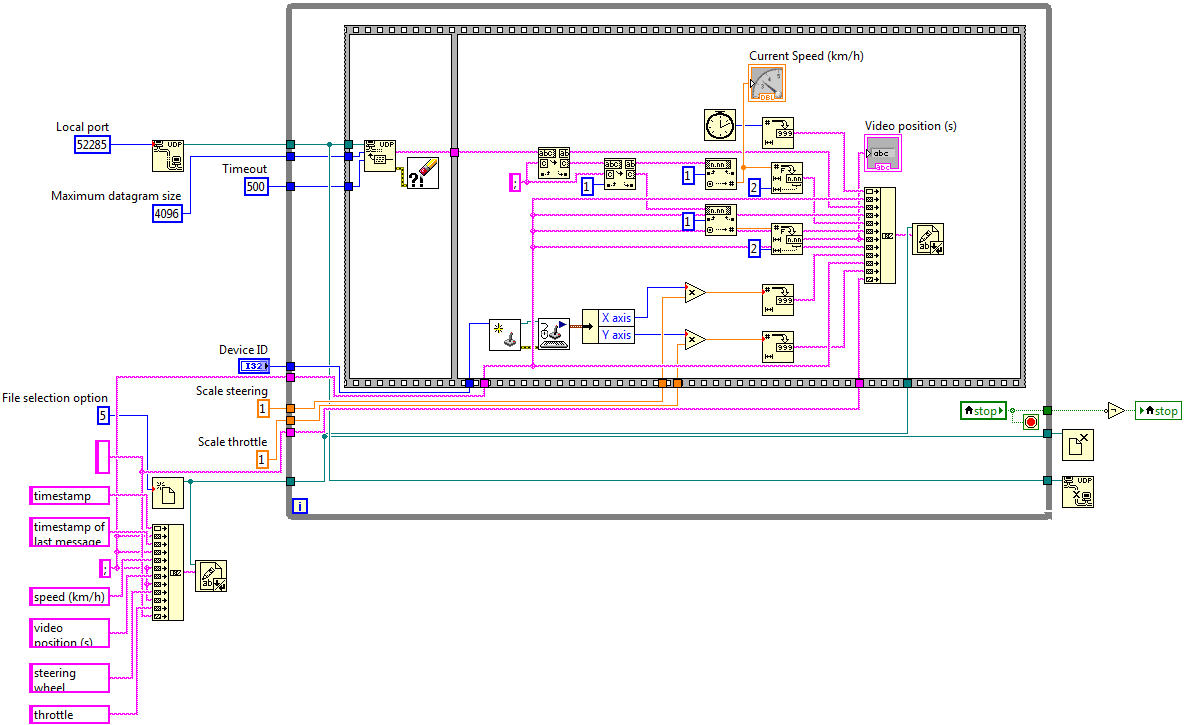
\includegraphics[angle=90,width=0.9\linewidth]{src/labview_screenshot_videoplayer_daten_empfangen.png}
\caption{LabVIEW: Daten empfangen} % Titel der Grafik
\label{labview_screenshot_videoplayer_daten_empfangen} % Labelname
\end{figure}

\newpage

\subsubsection{UDP-Listener}
Der UDP-Listener empfängt die Pakete, die von LabVIEW gesendet werden. Diese werden ausgepackt und die übermittelten Werte abgespeichert. Der UDP-Listener wird im Kapitel \ref{sec:udp-listener} genau dokumentiert.
\subsubsection{Hauptprogramm}
Das Hauptprogramm startet den MPlayer und den UDP-Listener. Der MPlayer wird, um ein Video abzuspielen, in einem eigenen Prozess gestartet und kann duch Aufrufe über die Standard-In-Pipe, wie im Listing \ref{start_mplayer} beschrieben, im Slavemodus gestartet werden. Wie der MPlayer im Videoplayer aufgerufen wird, kann dem Quellcode auf der beiliegenden DVD entnommen werden. 
\begin{lstlisting}[caption={Starten des MPlayers in einem eigenen Prozess}, label={start_mplayer}]
mplayer.exe -slave -hardframedrop -osdlevel 0 BeispielVideo.mp4
\end{lstlisting}
Der Parameter \textit{hardframedrop} dient der Erhöhung der Framerate. Es erlaubt dem Player bei hohen Abspielgeschwindigkeiten einzelne Bilder auszulassen um so eine höhere Framerate zu erzielen. Der \textit{osdlevel} Parameter bestimmt wieviel Information auf dem Bildschrim angezeigt wird. Der Level null unterdrückt alle Ausgaben.\\
In diesem Slavemodus nimmt der MPlayer Befehle die über die Standard-In-Pipe entgegen und schreibt seine Ausgabe in die Standard-Out-Pipe. Dazu werden die beiden Pipes des MPlayer-Prozesses im Hauptprogramm verfügbar gemacht und erlauben so eine Kommunikation der beiden Programme. 
\begin{lstlisting}[caption={Funktion zum Senden von Nachrichten an MPlayer}, label={mplayer_befehl}]
int sendMessage(const char* message)
{
	DWORD dwWritten;
	if(!WriteFile(stdInWr, message, strlen(message), &dwWritten, NULL))
	{
		fprintf(stderr, "Could not write to pipe.\n");
		return 1;
	}
	return 0;
}
\end{lstlisting}
Im Listing \ref{mplayer_befehl} quantifiziert \textit{speed} die Abspielgeschwindigkeit in der das Video abgespielt werden soll. 